\section{Approach}
    \label{sec:1}
\subsection{Architecture of the model}
To answer the self imposed question, a CNN will be used and fine tuned to achieve optimal classification performance on the chosen dataset. The architecture of the model can be subdivided into convolutional and dense blocks, whose number of convolutional and dense layers respectively are obtained in a hyperparameter search. Max pooling is used in each convolutional block to increase feature extraction from the data and reduce its dimensionality, while the each dense block contains a dropout layer to combat overfitting. The hyperparameter search was done using random search with a subsequent iterative bayesian search algorithm on the constrained parameter space. The architecture resulting from the hyperparameter search can be seen in \autoref{tab:arch}.
\begin{table}[H]
    \caption{The architecture of the neural network used for the final classification.}
    \vspace{0.2cm}
    \label{tab:arch}
    \centering
    \begin{adjustbox}{max width=\textwidth}
    \begin{tabular}{l|l|r}
        \toprule
        \multicolumn{3}{c}{\textbf{Architecture}} \\
        \midrule
        \textbf{Layer} & \textbf{Output Shape} & \textbf{Param \#} \\
        \midrule
        Input Layer & (None, 80, 96, 1) & 0 \\
        Conv2D & (None, 80, 96, 160) & 2,720 \\
        Conv2D & (None, 80, 96, 160) & 409,760 \\
        MaxPooling2D & (None, 40, 48, 160) & 0 \\
        Conv2D & (None, 40, 48, 160) & 409,760 \\
        Conv2D & (None, 40, 48, 160) & 409,760 \\
        MaxPooling2D & (None, 20, 24, 160) & 0 \\
        Conv2D & (None, 20, 24, 160) & 409,760 \\
        Conv2D & (None, 20, 24, 160) & 409,760 \\
        MaxPooling2D & (None, 10, 12, 160) & 0 \\
        Flatten & (None, 19200) & 0 \\
        Dense & (None, 448) & 8,602,048 \\
        Dropout & (None, 448) & 0 \\
        Dense & (None, 448) & 201,152 \\
        Dropout & (None, 448) & 0 \\
        Dense (Output) & (None, 6) & 2,694 \\
        \midrule
        \multicolumn{2}{l|}{\textbf{Total params}} & 10,857,414 \\
        \bottomrule
    \end{tabular}
    \end{adjustbox}
\end{table}
\noindent
The model has an input shape of 96 $\times$ 80, which is the image sized used for the final training due to time and computational constrains. It consists of 3 convolutional blocks followed by a flattening layer and 2 dense blocks with 448 dense units, based on the hyperparameter search. The max pooling size is 3 $\times$ 3 and the dropout rate is 0.5. Additional hyperparameters not directly related to the models architecture are found in \autoref{tab:params}.
\begin{table}[H]
    \caption{Hyperparameters and best Values}
    \vspace{0.2cm}
    \label{tab:params}
    \centering
    \begin{adjustbox}{max width=\textwidth}
    \begin{tabular}{l|r}
        \toprule
        \textbf{Hyperparameter}  & \textbf{Final Value} \\
        \midrule
        \textbf{filters} & 160 \\
        \textbf{kernel\_size}  & 4 \\
        \textbf{regularizer\_strength}  & 0.06 \\
        \textbf{conv\_activation}  & elu \\
        \textbf{dense\_activation} & elu \\
        \textbf{learning\_rate} & 0.00011 \\
        \bottomrule
    \end{tabular}
    \end{adjustbox}
\end{table}
\noindent
The architecture is optimized for feature extraction with a large amount of convolutional layers and is quite complex with a total of 10.857.414 trainable parameters. Additionally an earlier unoptimized CNN will be used for comparisons consisting of 2 convolutional blocks of three convolutional layers and otherwise same architecture with unoptimized hyperparameters. 
\subsection{Data preprocessing}
The preprocessing of the data is a crucial step for the success of the chosen method. With the .jpg images being of size (360, 640) and the amount of data being high, down-scaling of the images resolution and size becomes necessary for computation reasons. With this in mind, two methods were implemented, one doing a crop on the image to reduce background, and the other reducing the resolution of the image. 
The initial idea for the cropping was to use a face detection software to dynamically crop each picture according to the drivers face postition. This idea had to be dismissed as the face detection was not as reliable as initially hoped. With many drivers in the "Distraced" class looking to the side or down on their phone, the face detection algorithm started to detect faces in the background of the images, introducing a large bias into the dataset. 
An alternative method was then chosen, which crops 100 pixels from the left and right of every picture, significantly reducing the amount of background for the training of the CNN. A before and after comparison of the cropped images can be seen in \autoref{fig:comp1}
\begin{figure}[H]
    \centering
    \begin{subfigure}{0.48\textwidth}
        \centering
        \adjustbox{valign=c}{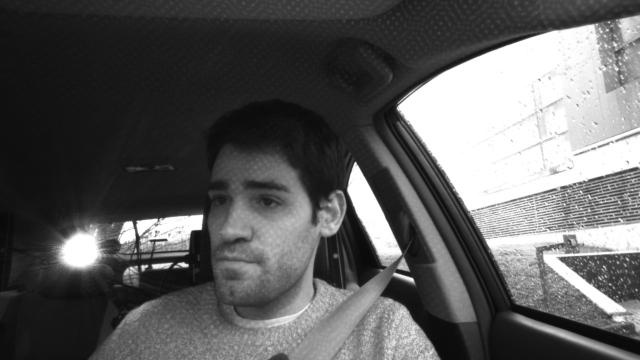
\includegraphics[width = \textwidth]{content/test1.jpg}}
    \end{subfigure}
    \hfill
    \begin{subfigure}{0.48\textwidth}
        \centering
        \adjustbox{valign=c}{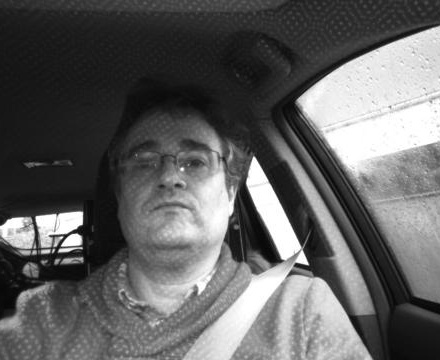
\includegraphics[width = \textwidth]{content/test2.jpg}}
    \end{subfigure}
    \caption{Comparison of the uncropped (left) and cropped (right) images.}
    \label{fig:comp1}
\end{figure}
\noindent
This is possible due to the camera position being relatively consistent throughout all images. A greater crop sometimes led to the faces or class relevant objects being cropped off and was thus not implemented. 
The cropped images were then scaled down to a resolution of 120 $\times$ 100 using the OpenCV \cite{opencv} library.
\section{Data augmentation and overfitting optimization}
    \label{sec:2}
This section will present the precautions taken to compensate for possible overfitting of the data and the data augmentation done to balance the amount of classes in the dataset.
\subsection{Data augmentation}
Classes like "Yawn" or "Drinking" have very few entry in contrast to the rest of the dataset, with relative amounts to the total dataset size being 
Safe driving: $41.59\%$,
Dangerous driving: $31.25\%$,
Distraced: $14.00\%$,
Sleepy driving: $6.59\%$,
Yawn: $3.68\%$,
Drinking: $2.89\%$ .
For this reason data augmentation is implemented to account for the drastic class imbalances.
The original approach for the augmentation process was to generate augmented data to fill up all classes to the number of entries of the largest class. This resulted in an immense amount of data being generated which could not be handled by the computational power avaiable. An alternative approach was then chosen, in which all classes are scaled to 2000 entries. This resulted in cutting off entries from the top three largest classes and only a minimal amount of data augmentation in the three smallest classes. 
The augmentation was conducted using the tensorflow.keras.preprocessing.image.ImageDataGenerator method, alongside a self implemented noise generator. The ImageDataGenerator does a random augmentation for each image based on initially set parameters. The augmentations applied to the images are shifts in width and height up to a value of 0.1, shear and zoom up to a value of 0.3 and 0.1 respectively and a possible vertical flip of the image. The noise generator applies random gaussian noise to each pixel, with the strength of the noise being random for each image. A total of 4047 augmented images were generated this way, while 6902 images were cut from the largest classes. 
\begin{figure}[H]
    \centering
    \begin{subfigure}{0.48\textwidth}
        \centering
        \adjustbox{valign=c}{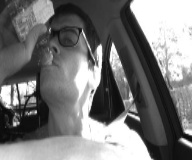
\includegraphics[width = \textwidth]{content/test_aug_1.jpg}}
    \end{subfigure}
    \hfill
    \begin{subfigure}{0.48\textwidth}
        \centering
        \adjustbox{valign=c}{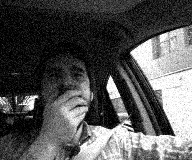
\includegraphics[width = \textwidth]{content/test_aug_2.jpg}}
    \end{subfigure}
    \caption{Two exemplary augmnted pictures with zoom and shear (right) and noise (left).}
    \label{fig:comp2}
\end{figure}
\noindent
Two exemplary augmented pictures can be seen in \autoref{fig:comp2}. The final CNN with optimized hyperparameters was then trained on both the original dataset and the augmented dataset with 2000 entries in each class. While the performance was roughly equal, the confusion matrices show the necessity of equally sized classes.
The confusion matrices for the training on both datasets can be seen in \autoref{fig:comp3}. 
\begin{figure}[H]
    \centering
    \begin{subfigure}{0.49\textwidth}
        \centering
        \adjustbox{valign=c}{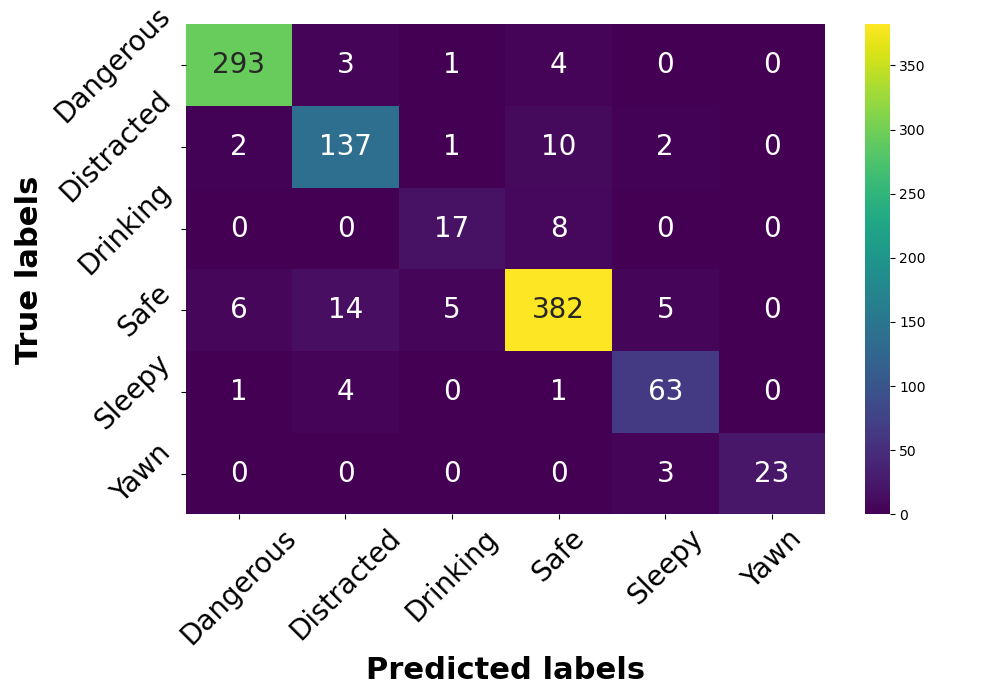
\includegraphics[width = \textwidth]{content/confusion_matrix_final_og.png}}
        \caption{Original dataset.}
    \end{subfigure}
    \hfill
    \begin{subfigure}{0.49\textwidth}
        \centering
        \adjustbox{valign=c}{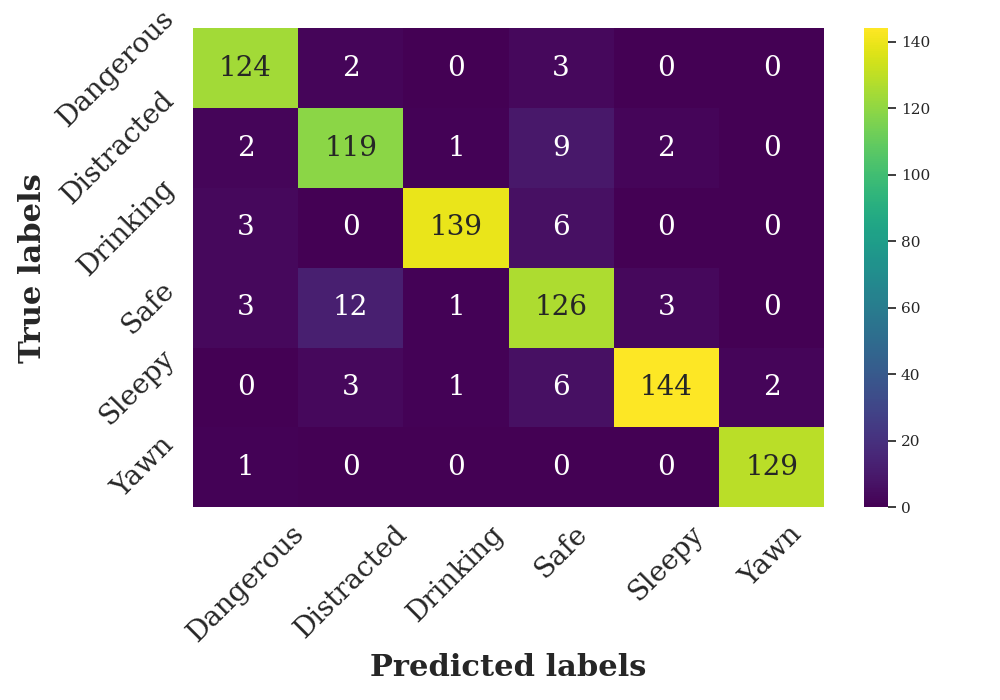
\includegraphics[width = \textwidth]{content/confusion_matrix_final_aug.png}}
        \caption{Augmented dataset.}
    \end{subfigure}
    \caption{Confusion Matrices on the test data of the original dataset (left) and the augmented dataset (right).}
    \label{fig:comp3}
\end{figure}
\noindent
The left confusion matrix of the original dataset shows a great amount of miss classification of pictures labeled "Drinking". This is not only due to an inacurate prediction, but also due to the small amount of entries labeled "Drinking" in the original test data, with a total of only 25 "Drinking" images. This shows a signigicantly decreased sensitivity in the low number of entries classes in comparison to the confusion matrix of the augmented dataset. For these reasons the augmented dataset was chosen to undergo a final 12-fold cross validation training in order to yield precise and generalized final results. The original dataset will still be used for a direct comparison to the alternative model to compare their performance on data with imbalanced classes.
\subsection{Overfitting optimization}
To avoid overfitting, several methods were implemented. The model itself contains 2 dropout layers with one in each dense block. These layers reduce overfitting as dropping out neurons during the training process regularizes the overtraining and increases the generalization of the model. Further regularization is introduced into the model by applying a L2 regularization to the loss function. This regularization penalizes large weights, leading to a reduction of the models complexity, which can be a reason for bad performance on unseen data.
The L2 regularization works by adding an additional term to the loss function which is then given by $$J(\theta) = \frac{1}{m} \sum_{i=1}^{m} L(y^{(i)}, h_\theta(x^{(i)})) + \frac{\lambda}{2m} \|\theta\|^2 \, .$$ The first term of the regularized loss function $J$ describes the traditional loss given the true true label $y^{\left(i\right)}$ and the models prediction $h_\theta\left(x^{\left(i\right)}\right)$ while the second term describes the regularization proportional to the squared sum of weights $\|\theta\|^2$, penalizing huge weights. Both the dropout rate and regularization strength are hyperparameters, whose optimal values are obtained in the hyperparameter optimization.
\begin{figure}[H]
    \centering
    \begin{subfigure}{0.49\textwidth}
        \centering
        \adjustbox{valign=c}{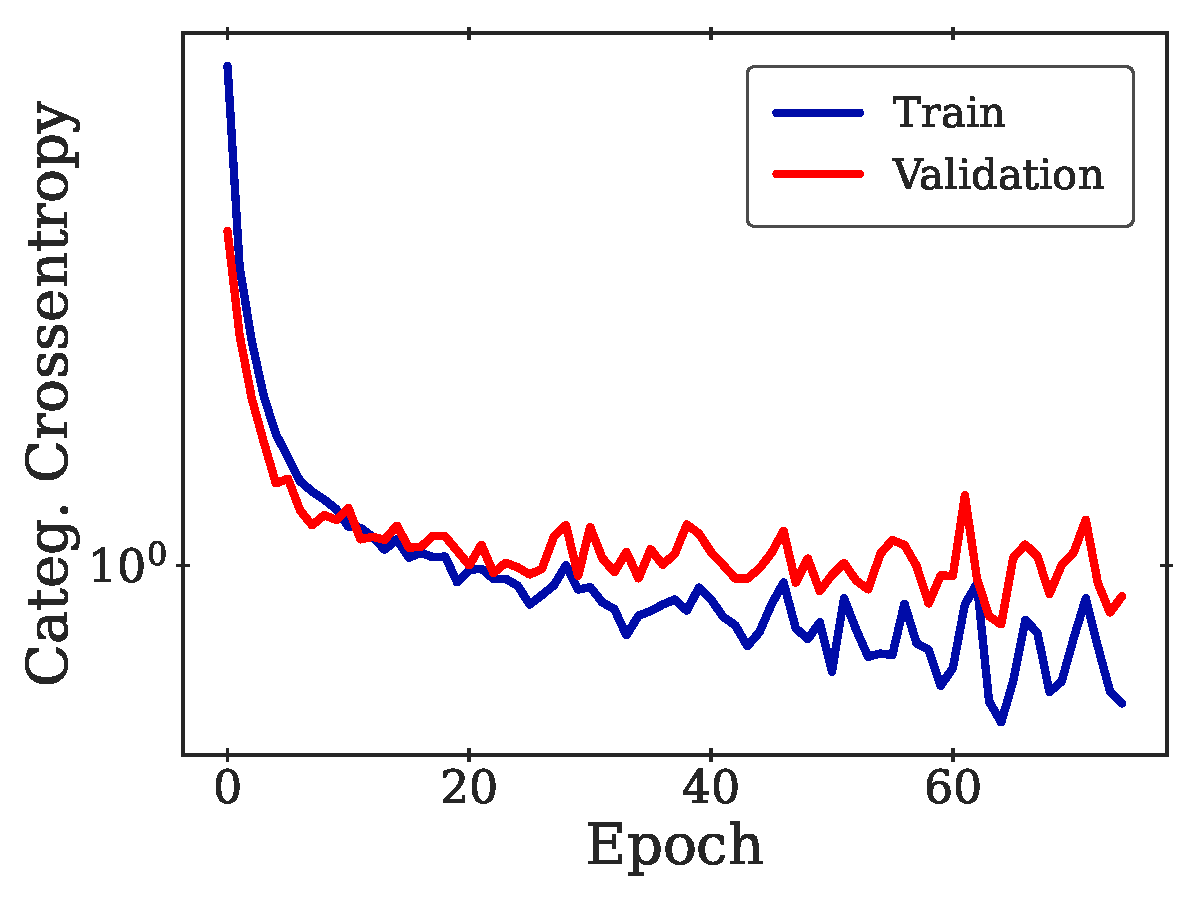
\includegraphics[width = \textwidth]{content/loss_bef_hyp.pdf}}
        \caption{Non optimal parameters without cross validation, training performed on 120 $\times$ 100 images.}
    \end{subfigure}
    \hfill
    \begin{subfigure}{0.49\textwidth}
        \centering
        \adjustbox{valign=c}{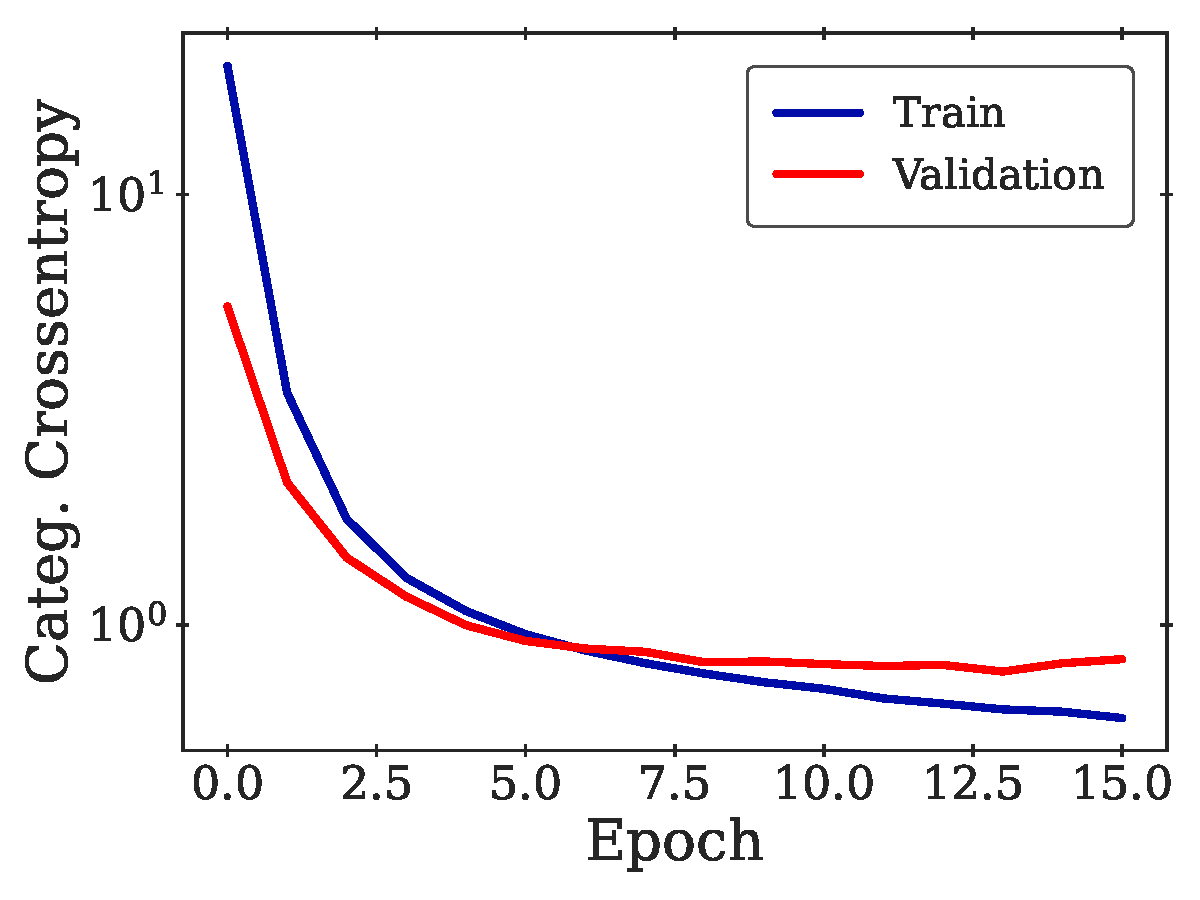
\includegraphics[width = \textwidth]{content/loss.pdf}}
        \caption{12-fold cross validated loss with optimal parameters, training on 96 $\times$ 80 images.}
        \label{fig:comp4b}
    \end{subfigure}
    \caption{Effects of the optimized hyperparameters on overfitting.}
    \label{fig:comp4}
\end{figure}
\noindent
\autoref{fig:comp4} shows the loss per epoch before and after the hyperparameter optimization. Without optimized parameters in these regularization methods, the loss on the left shows clear signs of overfitting and large oscillations. While the optimized loss on the right shows a much better result, it still runs into overfitting issues. This is due to the limited size of the augmented dataset chosen, with a larger dataset having too much computational cost. A larger dataset with equal image resolution would not run into overfitting as fast, but resulted in crashes on the used hardware or had to be aborted for time reasons. To combat the still existing overfitting, early stopping was implemented, which set the CNN's weights to the optimal values of a previous epoch, once a stagnation in the validation loss is detected. The effects of the early stopping can be clearly seen in \autoref{fig:comp4}, as the training in the right plot is stopped much earlier due to a clearer stagnation of the validation loss. This prevents the usage of an overfit model even though overfitting may still occur during the final training process.
Additionally, a 12-fold cross-validation was implemented during the final training process to further validate the generalization of the model, which was used for the training seen in \autoref{fig:comp4b}. This approach helps ensure that the model performs well on unseen data without sacrificing too much performance due to the limited size of the training set. 
\section{Results and comparison to alternative Method}
    \label{sec:3}
\subsection{Final performance of the CNN}

\subsection{Performance comparison to the Roboflow inference model}
The Roboflow inference model serving as the alternative method in this report is a pretrained model using the Roboflow object detection platform (cite). The Roboflow model is trained on the same dataset used for the CNN and thus a comparison will be made on the unbalanced original test data to avoid biases in the Roboflow model. For this purpose the optimized CNN is trained on the cropped and downscaled training and validation data, provided by the original dataset, and evaluated on the cropped and downscaled test data to be comparable with the Roboflow model evaluated on the unprocessed test data. 
The metrics of both models can be seen in \autoref{tab:comp_rob}
\begin{table}[htbp]
    \centering
    \caption{Performance comparison between Roboflow model including and excluding unidentified images and the self trained CNN.}
    \vspace{3pt}
    \label{tab:comp_rob}
    \begin{adjustbox}{max width=\textwidth}
    \begin{tabular}{l|cc|c|cc|c|cc|c}
        \toprule
        \textbf{Class} & \multicolumn{3}{c|}{\textbf{Roboflow, excl. unidentified}} & \multicolumn{3}{c|}{\textbf{Roboflow, incl. unidentified}} & \multicolumn{3}{c}{\textbf{CNN}} \\
        \cmidrule{2-10}
         & \textbf{Precision} & \textbf{Recall} & \textbf{Entries} & \textbf{Precision} & \textbf{Recall} & \textbf{Entries} & \textbf{Precision} & \textbf{Recall} & \textbf{Entries} \\
        \midrule
        Dangerous & 0.98 & 0.99 & 274 & 0.98 & 0.90 & 301 & 0.97 & 0.97 & 301 \\
        Distracted & 0.95 & 0.84 & 118 & 0.95 & 0.65 & 152 & 0.87 & 0.90 & 152 \\
        Drinking & 0.95 & 1.00 & 18 & 0.95 & 0.72 & 25 & 0.71 & 0.68 & 25 \\
        Safe & 0.94 & 0.96 & 331 & 0.94 & 0.77 & 412 & 0.94 & 0.93 & 412 \\
        Sleepy & 1.00 & 0.87 & 45 & 1.00 & 0.57 & 69 & 0.86 & 0.91 & 69 \\
        Yawn & 0.69 & 1.00 & 25 & 0.69 & 0.96 & 26 & 1.00 & 0.88 & 26 \\
        \midrule
        Macro avg & 0.92 & 0.94 & 811 & 0.79 & 0.65 & 985 & 0.89 & 0.88 & 985 \\
        Accuracy & 0.95 & \phantom{0} & 811 & 0.78 & \phantom{0} & 985 & 0.93 & \phantom{0} & 985 \\
        \bottomrule
    \end{tabular}
    \end{adjustbox}
\end{table}
\noindent 
The Roboflow model, accessed via the Roboflow API (cite), sometimes fails to classify a given image for unknown reasons. This results in higher metrics when excluded from the evaluation as portrayed in the left three columns of \autoref{tab:comp_rob}. For comparability the unidentified cases were included in the middle three columns of \autoref{tab:comp_rob} which results in much worse metrics on the test data, being outperformed by the CNN in the average metrics and accuracy. 
The confusion matrices shown in \autoref{fig:conf_comp} compare the results obtained by the CNN and the results of the Roboflow model when not excluding the unidentified images, represented by the extra column.
\begin{figure}[H]
    \centering
    \begin{subfigure}{0.49\textwidth}
        \centering
        \adjustbox{valign=c}{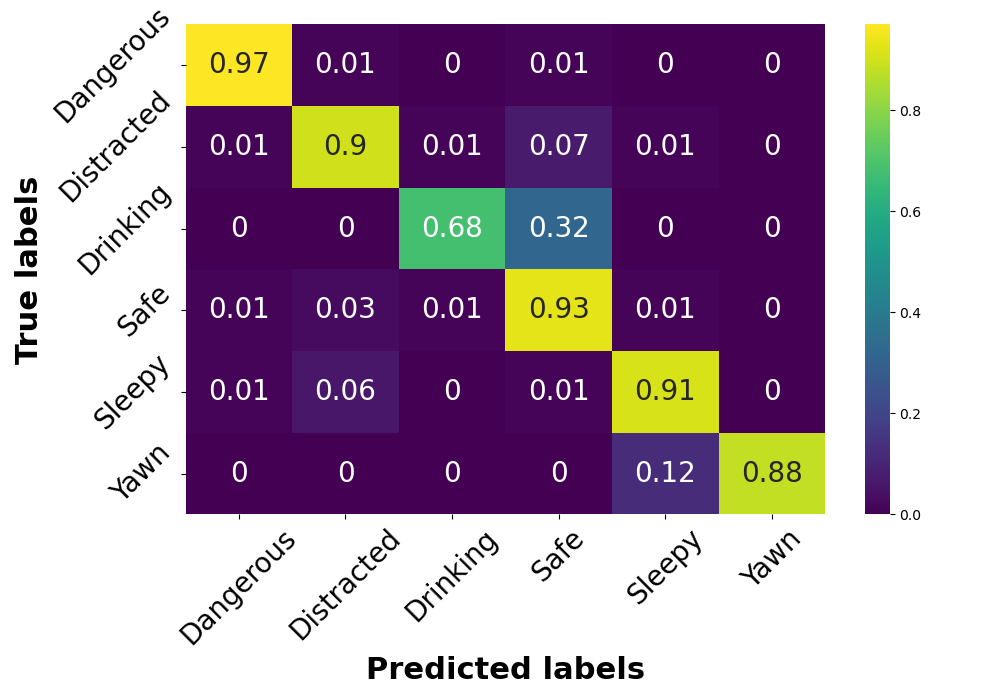
\includegraphics[width = \textwidth]{content/confusion_matrix_final_og_norm.png}}
        \caption{Confusion matrix of CNN on cropped and downscaled origial test data.}
    \end{subfigure}
    \hfill
    \begin{subfigure}{0.49\textwidth}
        \centering
        \adjustbox{valign=c}{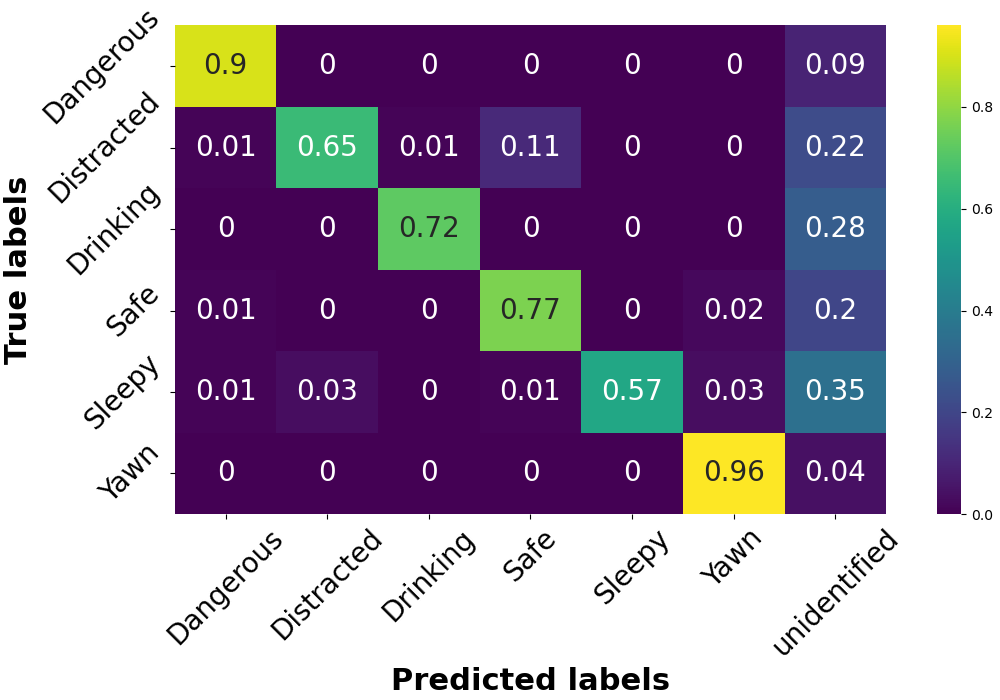
\includegraphics[width = \textwidth]{content/confusion_matrix_robo_unid.png}}
        \caption{Confusion matrix of Roboflow model on origial test data, including unidentified images.}
    \end{subfigure}
    \caption{Comparison of the confusion matrices.}
    \label{fig:conf_comp}
\end{figure}
\noindent
